\documentclass[t, 				             
			   final,
			   12pt, 				         
			   xcolor={usenames,dvipsnames}, 
			   table]{beamer}

% pacotes utilizados.
\usepackage[alf]{abntex2cite}
\usepackage{amsmath}
\usepackage[brazil]{babel}
\usepackage{booktabs}
\usepackage{caption}
\usepackage[utf8]{inputenc}
\usepackage{listings}
\usepackage{multicol}
\usepackage{multirow}
\usepackage{todo}


% configuração do tema
\usetheme[pageofpages=de,
          bullet=square,			
          titleline=true,				
          alternativetitlepage=true,			
          titlepagelogo=imagens/logo-puc,	
          watermarkheight=70px,		
          watermarkheightmult=4	
          ]{Torino}

\setbeamertemplate{sections/subsections in toc}[square]
\setbeamertemplate{bibliography item}[default]

\usecolortheme{freewilly}

% Block Environment
% -------------------------------
\setbeamertemplate {blocks}[default]
\setbeamercolor{block title}{fg=red!0!green!15!blue!85!, bg=red!33!green!37!blue!15!}
\setbeamercolor{block body}{fg=black, bg=red!32!green!33!blue!5}
\setbeamercolor{block title alerted}{fg=white, bg=red!40!black}
\setbeamercolor{block body alerted}{fg=black, bg=red!5!white}
\setbeamercolor{block title example}{fg=white, bg=green!40!black}
\setbeamercolor{block body example}{fg=black, bg=green!5!white}
\setbeamerfont{block title}{size=\scriptsize, series=\bfseries}


\definecolor{javared}{rgb}{0.6,0,0} % for strings
\definecolor{javagreen}{rgb}{0.25,0.5,0.35} % comments
\definecolor{javapurple}{rgb}{0.5,0,0.35} % keywords
\definecolor{javadocblue}{rgb}{0.25,0.35,0.75} % javadoc
 
\lstset{}

\lstdefinestyle{BashInputBasicStyle}{
	language=bash,
	basicstyle=\normalsize\ttfamily,
	columns=fullflexible,
	tabsize=2,
	showstringspaces=false,
	frame=single,
	inputencoding=utf8,
	rulecolor=\color{gray}
}

\lstdefinestyle{BashInputStyle}{
  language=bash,
  basicstyle=\normalsize\ttfamily,
  numbers=left,
  numberstyle=\tiny,
  numbersep=2pt,
  frame=tb,
  columns=fullflexible,
  tabsize=2,
  showstringspaces=false,
  commentstyle=\color{gray},
  inputencoding=utf8,
  rulecolor=\color{gray}
}

\lstdefinestyle{RubyInputStyle}{
    language=ruby,
    basicstyle=\scriptsize\ttfamily,
    keywordstyle=\color{javapurple},
    identifierstyle=\color{black},
    commentstyle=\color{javagreen},
	stringstyle=\color{blue},
    showstringspaces=false,
    numbers=left,
    numberstyle=\color{gray}\tiny,
    tabsize=3,
    extendedchars=\true,
    inputencoding=utf8,
%   frame=single, 
    columns=fixed,
    backgroundcolor=\color{red!32!green!33!blue!5}
}    
%  language=ruby,
%  basicstyle=\normalsize\ttfamily,
%  keywordstyle=\color{OrangeRed},
%  identifierstyle=\color{Turquoise},
%  commentstyle=\color{gray},
%  stringstyle=\color{YellowOrange},
%  numbers=left,
%  numberstyle=\tiny,
%  numbersep=2pt,
%  frame=tb,
%  columns=fullflexible,
%  backgroundcolor=\color{white!80},
%  linewidth=0.9\linewidth,
%  tabsize=2,
%  showstringspaces=false
%  inputencoding=utf8


\lstdefinestyle{JavaInputStyle}{
	language=Java,
	basicstyle=\ttfamily,
	keywordstyle=\color{javapurple}\bfseries,
	stringstyle=\color{javared},
	commentstyle=\color{javagreen},
	morecomment=[s][\color{javadocblue}]{/**}{*/},
	numbers=left,
	numberstyle=\tiny\color{black},
	numbersep=10pt,
	tabsize=2,
	showspaces=false,
	showstringspaces=false,
	frame=tb,
	columns=fullflexible,
	backgroundcolor=\color{white!80},
	linewidth=0.9\linewidth,
	inputencoding=utf8
}

\begin{document}
	\author{Luiz Alberto Ferreira Gomes}
\title{Aula 02: Ruby On Rails}
\subtitle{Laboratório de Projeto de Sistemas}
\institute{Curso de Ciência da Computação}
\date{\today}

	\begin{frame}[plain]
  \titlepage
\end{frame}
	\AtBeginSection[]
{
  \begin{frame}{Agenda}
    \tableofcontents[currentsection]
  \end{frame}
}
  	

    \section{Primeira Aplicação}
    %%-------------------------------------------------------------------------------------- Início
\begin{frame}[fragile,t]{Hora de Colocar a Mão na Massa}
	\begin{itemize}
		\item Conecte-se na máquina com o seu usuário e sua senha
		\begin{enumerate}
	    \item Inicie uma janela de terminal e digite no prompt:
	     \begin{lstlisting}[style=BashInputBasicStyle]
	     $ rails new my_app
	     \end{lstlisting}

	    \item Mude para o diretório da aplicao (RAILS.root)
	     \begin{lstlisting}[style=BashInputBasicStyle]
	     $ cd new my_app
	     \end{lstlisting}
    
	    \item Execute o servidor web embutido:
	    \begin{lstlisting}[style=BashInputBasicStyle]
	    $ rails s
	    \end{lstlisting}
	    
	    \item Abra uma janela do navegador e digite:
	     \begin{lstlisting}[style=BashInputBasicStyle]
	     $ http://localhost:3000
	     \end{lstlisting}
	  \end{enumerate}
	\end{itemize}
\end{frame}
    \include{rails-rest}
    
    \section{Ação Index}
	%%-------------------------------------------------------------------------------------- Início
\begin{frame}[allowframebreaks, t, fragile]{Ação: Index}
	\begin{itemize}
		\item Ação que recupera \alert{todas as postagens} do blog
		\item (Implicitamente) procura pelo template \alert{index.html.erb} para renderizar a resposta
		\begin{lstlisting}[style=RubyInputStyle, caption=controllers/posts\_controller.rb]
Class PostsController < ApplicationController
	def index
		@posts = Post.all
	end
end 
		\end{lstlisting}		
		\framebreak
		\item \alert{index.html.erb}:
		\begin{lstlisting}[style=RubyInputStyle, caption=views/posts/index.html.erb]
<h1>Posts</h1>
<table>
  <thead>
    <tr>
      <th>Title</th>
      <th>Body</th>
      <th colspan="3"></th>
    </tr>
  </thead>

  <tbody>
  <% @posts.each do |post| %>
    <tr>
      <td><%= post.title %></td>
      <td><%= post.body  %></td>
      <td><%= link_to 'Show', post %></td>
      <td><%= link_to 'Edit', edit_post_path(post) %></td>
      <td><%= link_to 'Delete', post, method: :delete, 
        data: { confirm: 'Tem certeza ?' } %></td>
    </tr>
  <% end %>
  </tbody>
</table>	
<%= link_to 'New Post', new_post_path %>	
\end{lstlisting}
	\end{itemize}	
\end{frame}
    %%%-------------------------------------------------------------------------------------- Início
\begin{frame}[allowframebreaks, t, fragile]{Ação: New}
	\begin{figure}[h!]
		\centering
		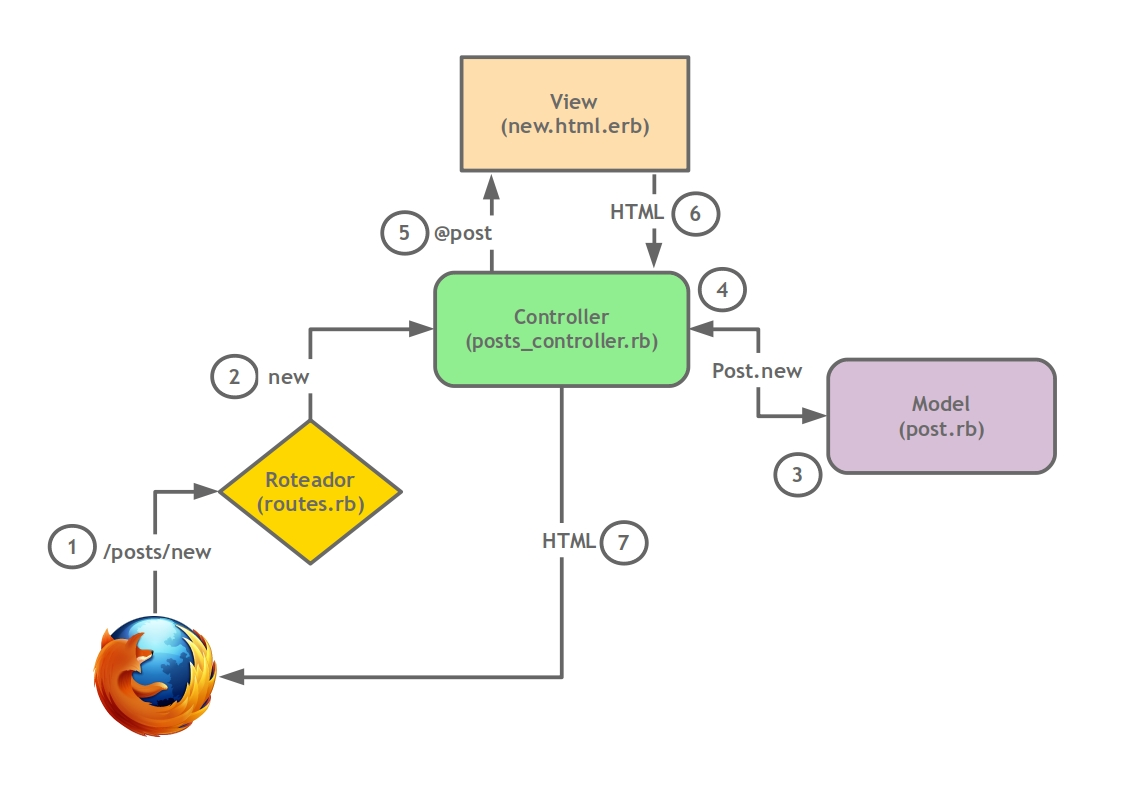
\includegraphics[width=0.75\textwidth]{imagens/mvc-action-new.jpg}
	\end{figure}
	\framebreak
	\begin{itemize}
		\item Um novo objeto \alert{@post} da classe \alert{Post} é instanciado 
		\item Procura pela visão \alert{new.html.erb} para renderizar a resposta
		\begin{lstlisting}[style=RubyInputStyle, caption=app/controllers/posts\_controller.rb]
Class PostsController < ApplicationController
  def new
    @post = Post.new 
  end 
end
		\end{lstlisting}
	\end{itemize}
\end{frame}

\begin{frame}[allowframebreaks, t, fragile]{Visão: New}
	\begin{itemize}
		\item Reinicie o servidor web e acesse a url \url{http:\\localhost:3000/posts/new}. Veja o erro que ocorreu.
		\item Implemente a visão \alert{new.html.erb}:
		\begin{lstlisting}[style=RubyInputStyle, caption=views/posts/new.html.erb]
<h1>Novo Post</h1>
<%= form_with model: @post, local: true do |form| %>
	<p>
		<%= form.label :title %><br>
		<%= form.text_field :title %>
	</p>
	
	<p>
		<%= form.label :body %><br>
		<%= form.text_area :body %>
	</p>
	
	<p>
		<%= form.submit %>
	</p>
<% end %>	
		\end{lstlisting}
	\end{itemize}	
\end{frame}
    %%%-------------------------------------------------------------------------------------- Início
\begin{frame}[allowframebreaks, t, fragile]{Ação: Create}
  \begin{figure}[h!]
		\centering
		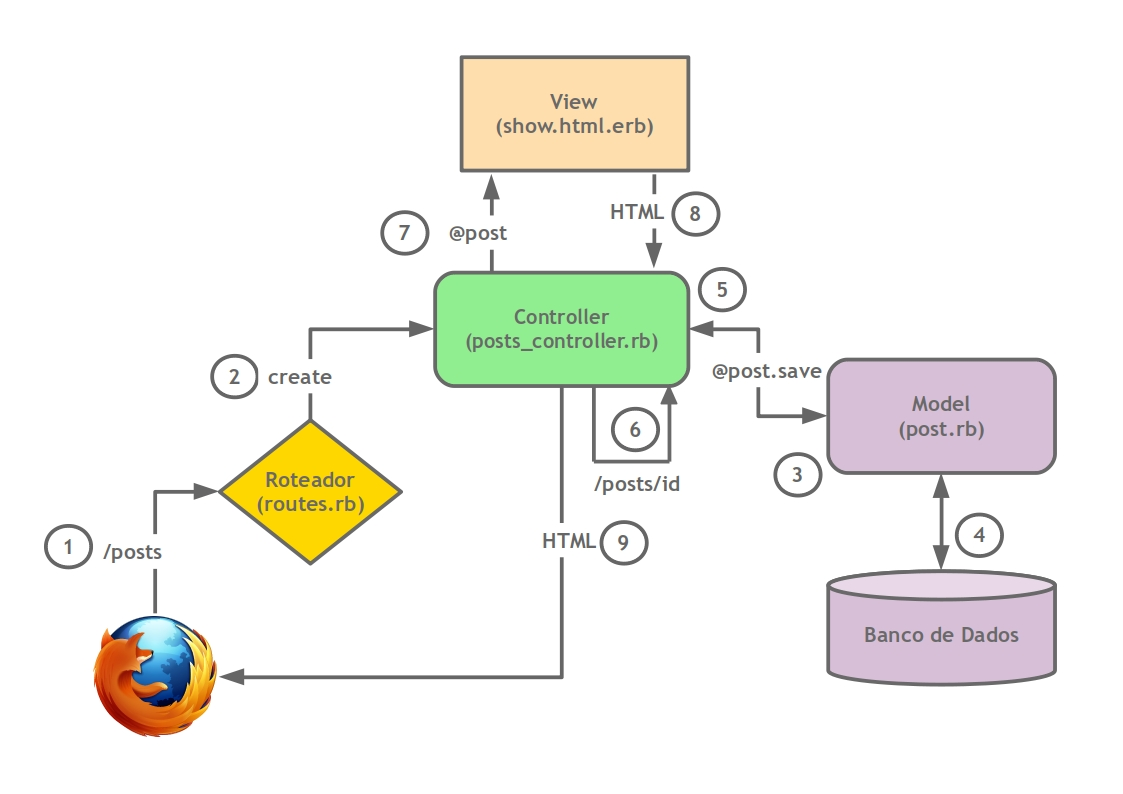
\includegraphics[width=0.75\textwidth]{imagens/mvc-action-create.jpg}
	\end{figure}
	\framebreak
  \begin{itemize}
		\item Um novo objeto \alert{@post} da classe \alert{Post} é criado com os parâmetros que foram passados pelo 
			formulário \alert{new}
		\item Tenta \alert{salvar} o objeto \alert{@post} no \alert{banco de dados}
%		\item Se sucesso, redireciona para o template \alert{show}
%		\item Se insucesso, renderiza o template \alert{new} novamente
		\begin{lstlisting}[style=RubyInputStyle, caption=controllers/posts\_controller.rb]
class PostsController < ApplicationController
  def new
      @post = Post.new
  end

  def create 
      @post = Post.new(post_params)
      
      @post.save
      redirect_to @post
  end

private 
  def post_params 
    params.require(:post).permit(:title, :body)
  end
end          
		\end{lstlisting}		
		\begin{itemize}
			\item a linha 15 implementa \alert{strong parameters} para aumentar a segurança da aplicação
    \end{itemize}
    \item Como a ação {\bf Show} ainda não foi implementada, ocorrerá uma erro quando
    o botão {\bf Submit} for pressionado.
	\end{itemize}	
\end{frame}
    %%%-------------------------------------------------------------------------------------- Início
\begin{frame}[allowframebreaks, t, fragile]{Ação: Show}
	\begin{figure}[h!]
		\centering
		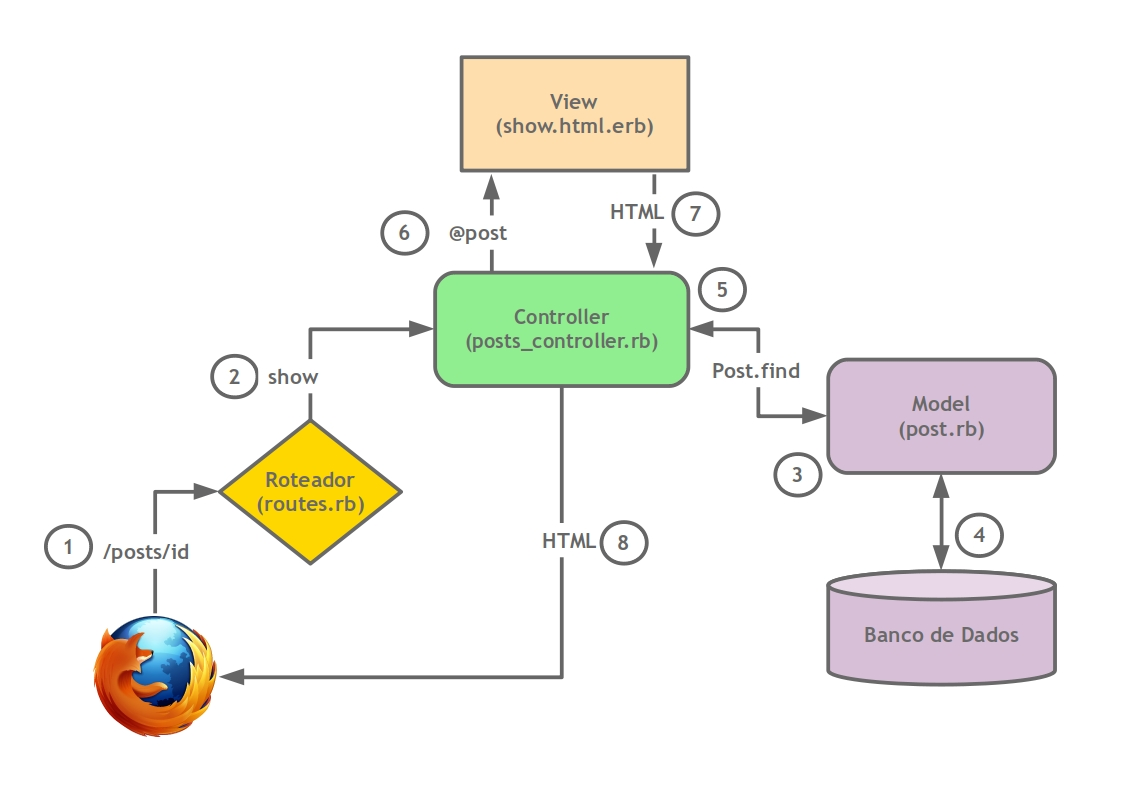
\includegraphics[width=0.75\textwidth]{imagens/mvc-action-show.jpg}
	\end{figure}
	\framebreak
	\begin{itemize}
		\item Recupera \alert{uma} postagem específica no parâmetro \alert{id} passado como parte da URL
		\item (Implicitamente) procura pelo \alert{show.html.erb} para renderizar a resposta
		\begin{lstlisting}[style=RubyInputStyle, caption=controllers/posts\_controller.rb]
class PostsController < ApplicationController
	def show 
		@post = Post.find(params[:id])
	end

	def new
		@post = Post.new
	end

	def create 
		@post = Post.new(post_params)
		
		@post.save
		redirect_to @post
	end
private 
	def post_params 
		params.require(:post).permit(:title, :body)
	end
end
		\end{lstlisting}
	\end{itemize}	
\end{frame}

%%-------------------------------------------------------------------------------------- Início
\begin{frame}[allowframebreaks, t, fragile]{Visão: Show}
	\begin{itemize}
		\item Implemente a visão \alert{show.html.erb}:
		\begin{lstlisting}[style=RubyInputStyle, caption=views/posts/show.html.erb]
<p>
	<strong>Title:</strong>
	<%= @post.title %>
</p>
<p>
<strong>Body:</strong>
	<%= @post.body %>
</p>
		\end{lstlisting}		
	\end{itemize}	
\end{frame}
    
\begin{frame}[t, fragile]{Database Console}
	\begin{itemize}
		\item O comando \alert{rails db} fornece uma console para acesso aos bancos dados
		MySQL, PostgreSQL e SQLite.
	\end{itemize}
	
	\begin{lstlisting}[style=BashInputBasicStyle, basicstyle=\tiny\ttfamily,  keepspaces=true]
		$ rails db
		SQLite version 3.8.7.1 2014-10-29 13:59:56
		Enter ".help" for usage hints.
		sqlite> .headers on
		sqlite> .mode columns
		sqlite> select * from posts;
		id          title             body            created_at                  updated_at                
		----------  ----------------  --------------  --------------------------  --------------------------
		5           A Linguagem Ruby  Ruby e legal.  2016-04-30 22:45:20.636363  2016-04-30 22:45:20.636363
		sqlite> 
	\end{lstlisting}
	
	\begin{itemize}
		\item Dica: utilize \alert{headers on} e \alert{mode coluns}
	\end{itemize}
	
\end{frame}

\begin{frame}[allowframebreaks, t, fragile]{Hora de Colocar a Mão na Massa}
	\begin{itemize}
		\item Inicialize \alert{na pasta da aplicação} a console do banco de dados e
		configure a sua exibição:
		\begin{lstlisting}[style=BashInputBasicStyle]
			$ rails db
			sqlite> .headers on
			sqlite> .mode columns
		\end{lstlisting}
		
		\item Exiba os colunas da tabela \verb|posts|:
		\begin{lstlisting}[style=BashInputBasicStyle]
			sqlite> .schema posts
		\end{lstlisting}
		
		\framebreak
		\item Exiba todos os \verb|posts|:
		\begin{lstlisting}[style=BashInputBasicStyle]
			sqlite> SELECT * FROM posts;
		\end{lstlisting}
		
		\item Exiba todos os \verb|posts| ordenados pelo título (title):
		\begin{lstlisting}[style=BashInputBasicStyle]
			sqlite> SELECT * FROM posts ORDER BY title;
		\end{lstlisting}
		
		\item Exiba um \verb|post|:
		\begin{lstlisting}[style=BashInputBasicStyle]
			sqlite> SELECT * FROM posts LIMIT 1
		\end{lstlisting}
		
		\item Exiba o \verb|post| cujo \verb|id| é 2:
		\begin{lstlisting}[style=BashInputBasicStyle]
			sqlite> SELECT * FROM posts WHERE id=2;
		\end{lstlisting}
	\end{itemize}
\end{frame}
    \begin{frame}[allowframebreaks, t, fragile]{Rails Console}
	\begin{itemize}
		\item Inicialize \alert{na pasta da aplicação} a console do Rails (não a do banco de dados):
		\begin{lstlisting}[style=BashInputBasicStyle]
			$ rails c
		\end{lstlisting}
		
		\item Exiba os atributos da classe \verb|Post|:
		\begin{lstlisting}[style=BashInputBasicStyle]
			irb(main):004:0> Post.column_names
		\end{lstlisting}
		
		\item Crie um novo \verb|post| e salve no banco de dados:
		\begin{lstlisting}[style=BashInputBasicStyle]
			irb(main):005:0> p1 = Post.new
			irb(main):006:0> p1.title="Rails is Cool!"
			irb(main):007:0> p1.body="Rails is really Cool..."
			irb(main):008:0> p1.save
		\end{lstlisting}
		
		\item Exiba todos os \verb|posts|:
		\begin{lstlisting}[style=BashInputBasicStyle]
			irb(main):007:0> Post.all
		\end{lstlisting}
		
		\item Exiba todos os \verb|posts| ordenados pelo título (title):
		\begin{lstlisting}[style=BashInputBasicStyle]
			irb(main):007:0> Post.all.order(title: :asc)
		\end{lstlisting}
		
		\item Exiba um \verb|post|:
		\begin{lstlisting}[style=BashInputBasicStyle]
			irb(main):007:0> Post.first
		\end{lstlisting}
		
		\item Exiba o \verb|post| cujo \verb|id| é 2:
		\begin{lstlisting}[style=BashInputBasicStyle]
			irb(main):007:0> Post.find_by(id: 2)
		\end{lstlisting}
		
		\item Atualize o título do primeiro \verb|post|:
		\begin{lstlisting}[style=BashInputBasicStyle]
			irb(main):007:0> p1=Post.first
			irb(main):008:0> p1.update(title: "Rails rules!")
		\end{lstlisting}
		
		\item Remova do primeiro \verb|post|:
		\begin{lstlisting}[style=BashInputBasicStyle]
			irb(main):007:0> p1=Post.first
			irb(main):008:0> p1.destroy
		\end{lstlisting}
		
	\end{itemize}
\end{frame}

    \section{Versionando a Primeira Aplicação}
    %-------------------------------------------------------------------------------------- Início
\begin{frame}[allowframebreaks, t, fragile]{Controle Automatizado de Versão}
	\begin{itemize}
		\item GitHub
		\item git
		\item git init
		\item git add 
		\item git commit
		\item git remote
		\item git push
	\end{itemize}
\end{frame}
%-------------------------------------------------------------------------------------- Início
\begin{frame}[fragile, plain, c]{GitHub}
    \begin{center}
        \begin{figure}[h]
            
\includegraphics[width=0.5\textwidth]{imagens/github.png}
            \caption{www.github.com}
        \end{figure}
	\end{center}
\end{frame}
%-------------------------------------------------------------------------------------- Início
\begin{frame}[fragile, plain, c]{git}
    \begin{center}
        \begin{figure}[h]
            
\includegraphics[width=0.5\textwidth]{imagens/git.png}
            \caption{https://git-scm.com/}
        \end{figure}
	\end{center}
\end{frame}
%-------------------------------------------------------------------------------------- Início
\begin{frame}[fragile, plain, c]{git $+$ GitHub}
    \begin{center}
        \begin{figure}[h]
            
\includegraphics[width=0.5\textwidth]{imagens/git_github.jpeg}
            \caption{https://git-scm.com/}
        \end{figure}
	\end{center}
\end{frame}
    
%%-------------------------------------------------------------------------------------- Início
\begin{frame}[allowframebreaks, fragile,t]{Hora de Colocar a Mão na Massa}
	\begin{enumerate}
        \item Reinicie o repositório local 
		\begin{lstlisting}[style=BashInputBasicStyle]
			$ git init
		\end{lstlisting}

        \item Efetive as mudanças realizadas no repositório local:  		
        \begin{lstlisting}[style=BashInputBasicStyle]
			$ git add .
			$ git commit -m "commit inicial"
		\end{lstlisting}

		\item Registre as alterações no repositório remoto:
        \begin{lstlisting}[style=BashInputBasicStyle]
$ git branch -M main
$ git remote add origin https://endereco/do/seu/repositorio.git
$ git push -u origin main
		\end{lstlisting}
	\end{enumerate}
\end{frame}    
    
    %\section{Ação Edit}
	%%%-------------------------------------------------------------------------------------- Início
\begin{frame}[t, fragile]{Ação: Edit}
	\begin{itemize}
		\item Recupera uma postagem específica no parâmetro \alert{id} passado como parte da URL
		\item (Implicitamente) procura pelo \alert{edit.html.erb} para renderizar a resposta
		\begin{lstlisting}[style=RubyInputStyle, caption=controllers/posts\_controller.rb]
Class PostsController < ApplicationController
  def edit 
    @post = Post.find(params[:id])
  end 
		\end{lstlisting}		
	\end{itemize}	
\end{frame}
    %\section{Ação Partials}
	%%%-------------------------------------------------------------------------------------- Início
\begin{frame}[allowframebreaks, t, fragile]{Partials}
	\begin{itemize}
		\item Rails encoraja o princípio \alert{DRY}	
		\item O laioute da aplicação é mantida em um único local no arquivo \alert{application.html.erb}
		\item O código comum dos templates ser reutilizado em \alert{múltiplos templates}
		\item Por exemplo, os formulários do \alert{edit} e do \alert{new} - são realmente muito diferentes ?
		\item Partials são similares aos templates regulares, mas ele possuem capacidades mais \alert{refinadas}
		\item Nomes de partials começam com \alert{underscore} (\_) 
		\item Partials são renderizados com \alert{render 'partialname'} (sem underscore)
		%\item \alert{render} também aceita um segundo argumento, um hash com as variáveis locais utilizadas no partial
		%\item Similar a passagem de variáveis locais, o \alert{render} pode receber um objeto
		%\item \alert{$<$\%= render @post \%$>$} renderizara \alert{app/views/posts/\_posts.html.erb} com o conteúdo da variavel @post
\framebreak
		%\item \alert{$<$\%= render @posts \%$>$} renderiza uma coleção e é equivalente a:
		%\begin{lstlisting}[style=RubyInputStyle, caption=controllers/posts\_controller.rb]
		%	<% @posts.each do |posts| %> 
		%		<%= render post %>
		%	<% end %>
		%\end{lstlisting}		
		%\framebreak
		\item \alert{\_form.html.erb}
		\begin{lstlisting}[style=RubyInputStyle, caption=views/posts/\_form.html.erb]
<%= form_with  model: @post, local: true do |form| %>
	<p>
		<%= form.label :title %><br>
		<%= form.text_field :title %>
	</p>
	
	<p>
		<%= form.label :body %><br>
		<%= form.text_area :body %>
	</p>
	
	<p>
		<%= form.submit %>
	</p>
<% end %>	
<%= link_to 'Back', posts_path %>
		\end{lstlisting}
	\end{itemize}	
\end{frame}



    %\section{Visão Edit}
	%%%-------------------------------------------------------------------------------------- Início
\begin{frame}[allowframebreaks, t, fragile]{View: Edit}
	\begin{itemize}
		\item \alert{edit.html.erb}:
		\begin{lstlisting}[style=RubyInputStyle, caption=view/posts/edit.html.erb]
			<h1>Edit Post</h1>
			<%= render 'form' %>
		\end{lstlisting}		
	\end{itemize}	
\end{frame}
    %\section{Visão Update}
	%%%-------------------------------------------------------------------------------------- Início
\begin{frame}[allowframebreaks, t, fragile]{Ação: Update}
	\begin{itemize}
		\item Recupera um objeto \alert{post} utilizando o parâmetro \alert{id}	
		\item Atualiza o objeto \alert{post} com os parâmetros que foram passados pelo
			formulário \alert{edit}
		\item Tenta \alert{atualizar} o objeto no \alert{banco de dados}
		%\item Se sucesso, redireciona para o template \alert{show}
		%\item Se insucesso, renderiza o template \alert{edit} novamente
		\begin{lstlisting}[style=RubyInputStyle, caption=posts\_controller.rb]
Class PostsController < ApplicationController
  def update
    @post = Post.find(params[:id])
	@post.update(post_params)
	redirect_to @post
  end
  ...
  	\end{lstlisting}				
	\end{itemize}	
\end{frame}



    %\section{Visão Destroy}
	%%%-------------------------------------------------------------------------------------- Início
\begin{frame}[allowframebreaks, t, fragile]{Ação: Destroy}
	\begin{itemize}
		\item Remove uma postagem específica pelo parâmetro \alert{id} passado como parte da URL
		\begin{lstlisting}[style=RubyInputStyle, caption=posts\_controller.rb]
Class PostsController < ApplicationController
  def destroy
    @post = Post.find(params[:id])
	@post.destroy
	redirect_to posts_path
  end 
		\end{lstlisting}		
	\end{itemize}	
\end{frame}
    %\section{Controle de Versão}
	%%%-------------------------------------------------------------------------------------- Início
\begin{frame}[allowframebreaks, fragile,t]{Hora de Colocar a Mão na Massa}
	\begin{enumerate}
		\item Registre as mudanças realizadas no repositório local:
		\begin{lstlisting}[style=BashInputBasicStyle]
			$ git add .
		\end{lstlisting}

        \item Efetive as mudanças realizadas no repositório local:  		
        \begin{lstlisting}[style=BashInputBasicStyle]
			$ git commit -m "#1: manutencao de posts"
		\end{lstlisting}

		\item Registre as alterações no repositório remoto:
		\begin{lstlisting}[style=BashInputBasicStyle]
			$ git push -u origin master
		\end{lstlisting}
	\end{enumerate}
\end{frame}
    
    \section{Para Saber Mais}
	%%-------------------------------------------------------------------------------------- Início
\begin{frame}[fragile,t]{Para Saber Mais}
  \begin{itemize}
    \item \url{https://www.ruby-lang.org/en/}
    \begin{itemize}
     \item referência oficial da linguagem Ruby onde a toda a sua documentação está disponível
	para ser consultada.
    \end{itemize}

    \item \url{http://rubyonrails.org/}
    \begin{itemize}
     \item referência oficial do framework Rails onde a toda a sua documentação está disponível
	para ser consultada.
    \end{itemize}
    
    \item \url{http://www.codecademy.com/pt/tracks/ruby}
    \begin{itemize}
     \item curso iterativo em portugês sobre a linguagem Ruby.
    \end{itemize}

	\item \url{https://gorails.com/setup/ubuntu/16.04}
	\begin{itemize}
		\item guia para instalação do Ruby on Rails no Ubuntu e no Mac OSX.
	\end{itemize}
  \end{itemize}
  
  
\end{frame}
\end{document}
